\documentclass[conference,a4paper]{IEEEtran}

\usepackage[utf8]{inputenc}
\usepackage[T1]{fontenc}
\usepackage[spanish,es-tabla]{babel}
\usepackage{graphicx}
\usepackage{booktabs}
\usepackage{amsmath}
\usepackage{url}
\usepackage{cite}
\usepackage{hyperref}

\graphicspath{{figures/}}

\title{Ocupación de plazas y conteo de accesos en un estacionamiento con YOLO11}

\author{%
\IEEEauthorblockN{Trabajo práctico}
\IEEEauthorblockA{Visión por Computadora II\\
CEIA, Facultad de Ingeniería, Universidad de Buenos Aires}
}

\begin{document}
\maketitle

\begin{abstract}
Este trabajo describe un prototipo que estima la ocupación de un estacionamiento con dos cámaras. La cámara interna usa un detector YOLO11 afinado sobre PKLot y cuenta plazas libres y ocupadas. La cámara de acceso no se reentrena: un YOLO11s de COCO, el seguidor ByteTrack y el cruce de una línea virtual distinguen ingresos de egresos. Se comparó YOLO11n con YOLO11s durante 20 épocas, con un corte por día de captura. En el test, YOLO11n obtuvo mAP50 de 0,914 y YOLO11s de 0,891, con latencias de 9,83\,ms y 9,52\,ms por frame en una RTX 4060 Ti. Se despliega el nano. En un video de tránsito el acceso contó 3 ingresos y 1 egreso.
\end{abstract}

\begin{IEEEkeywords}
estacionamiento, detección de objetos, YOLO, seguimiento, PKLot
\end{IEEEkeywords}

\section{Introducción}
Encontrar lugar para estacionar sigue siendo un problema operativo: el conductor recorre pasillos y el operador no sabe, en el momento, cuántas plazas quedan. Una cámara fija ya mira el predio. El prototipo convierte esa imagen en dos números: plazas libres u ocupadas, y vehículos que entran o salen.

El objetivo es un sistema que corra sobre video, justifique la arquitectura con una métrica y no se quede en clasificar la foto entera. Cada frame de un estacionamiento contiene decenas de plazas. Hace falta una caja por plaza.

Como caso reciente del mismo problema, Pokhrel y Dao compararon en 2025 distintos backbones dentro de YOLOv8 sobre PKLot y mostraron que la elección de la red cambia el equilibrio entre precisión y costo \cite{pokhrel2025yolov8pklot}. Ese trabajo se queda en la ocupación de las plazas. El prototipo de este paper agrega una segunda cámara, de entrada y salida, y compara dos tamaños de YOLO11 \cite{jocher2024yolo11} con un corte por día, no un cambio de backbone. El dataset de base sigue siendo PKLot \cite{almeida2015pklot}.

\section{Metodología}
La Fig.~\ref{fig:diagrama} resume las dos ramas. No se fusionan en un único contador: la cámara interna mira las plazas y la de acceso mira el flujo. El enlace entre ambas es de interpretación. Un ingreso resta uno al cupo libre y un egreso suma uno, pero ese delta no reemplaza la detección de las plazas.

\begin{figure*}[t]
\centering
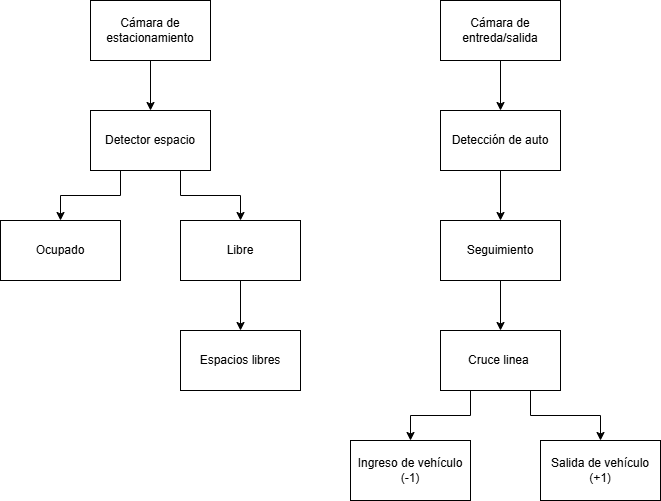
\includegraphics[width=0.92\textwidth]{diagrama.png}
\caption{Las dos cámaras del prototipo. La interna clasifica plazas. La de acceso cuenta el sentido del cruce.}
\label{fig:diagrama}
\end{figure*}

\subsection{Plazas}
PKLot publica fotos de 1280$\times$720 de estacionamientos de UFPR y PUCPR, con un polígono por plaza y un atributo de ocupación \cite{almeida2015pklot}. Esas anotaciones se convierten a cajas YOLO: el rectángulo eje-alineado que encierra el contorno, normalizado, con clase 0 para libre y 1 para ocupada. El archivo original pesa 4,6\,GB. Sin clave de Roboflow se usó el espejo público del mismo archivo. El export de Roboflow del mismo dataset queda como vía alternativa \cite{pokhrel2025yolov8pklot}.

Fotos tomadas a cinco minutos de diferencia son casi iguales. Un corte aleatorio pondría vecinos en train y en test y empujaría el mAP hacia arriba. Por eso el corte es por día de captura, con semilla fija: 70\,\% de los días para entrenar (8864 imágenes), 15\,\% para validar (1814) y 15\,\% para test (1738).

Se afinan YOLO11n y YOLO11s, ambos inicializados con pesos de COCO, durante 20 épocas, imágenes de 640, batch 8, paciencia 5 y precisión mixta, en una RTX 4060 Ti. La paciencia no cortó ninguna de las dos corridas: las dos llegaron a la época 20. YOLO de una etapa \cite{redmon2016yolo} evita la red de propuestas de Faster R-CNN \cite{ren2015faster}. Esa segunda etapa mejora la localización en varios benchmarks, pero en video de vigilancia el presupuesto es el tiempo por frame. La comparación empírica de este trabajo es entre dos tamaños de la misma familia, que es lo que se puede medir en la misma GPU y el mismo split.

La regla de selección se fijó antes de mirar el test: se elige el mayor mAP50 entre los modelos cuya latencia media no supere 1,5 veces la del más rápido. La latencia es el tiempo de \texttt{predict} sobre 40 imágenes del test, con tres de calentamiento, sincronizando la GPU.

\subsection{Accesos}
El detector de vehículos es YOLO11s preentrenado en COCO. No se lo vuelve a entrenar. Se conservan las clases auto, camión, colectivo y moto. ByteTrack \cite{zhang2022bytetrack} asigna un identificador persistente. El punto que cruza la línea es el centro de la caja. Hay cruce si ese centro cambia de semiplano respecto de la recta y, en ese frame, queda a lo sumo a 18 píxeles del segmento. Cada identificador se cuenta una sola vez. Pasar del semiplano positivo al negativo es un ingreso (delta $-1$); el sentido contrario es un egreso (delta $+1$). El umbral y el sentido viven en un archivo de configuración, porque dependen de dónde esté montada la cámara.

\section{Resultados}
La Tabla~\ref{tab:test} es el test de días no vistos. YOLO11n queda por encima en mAP50 (0,914 contra 0,891) con una latencia indistinguible a efectos prácticos (9,83\,ms contra 9,52\,ms). Las dos latencias están muy por debajo del factor 1,5, así que la regla se decide por el mAP50 y elige el nano. La precisión y el recall casi no se mueven.

\begin{table}[t]
\caption{Test de PKLot, días no usados en el entrenamiento. Latencia media de inferencia en una RTX 4060 Ti.}
\label{tab:test}
\centering
\begin{tabular}{lcccc}
\toprule
Modelo & mAP50 & mAP50-95 & Precisión & ms \\
\midrule
YOLO11n & 0,914 & 0,857 & 0,887 & 9,83 \\
YOLO11s & 0,891 & 0,856 & 0,889 & 9,52 \\
\bottomrule
\end{tabular}
\end{table}

El promedio esconde un desbalance. El test tiene 124468 plazas: 96133 libres y 28335 ocupadas. En YOLO11n la clase libre llega a precisión 0,995, recall 0,917 y mAP50 0,957. La clase ocupada llega a precisión 0,780, recall 1,000 y mAP50 0,870 (Tabla~\ref{tab:clases}). Casi no se pierde una plaza ocupada, pero una de cada cinco cajas marcadas como ocupadas no lo está. Para quien busca lugar, ese error esconde un espacio libre. El error inverso, mandar un auto a una plaza tomada, es el recall de la clase libre: 0,917, o sea que algunas plazas vacías no se recuperan.

\begin{table}[t]
\caption{Test de YOLO11n por clase. El mAP50 global de 0,914 pondera mucho más las plazas libres.}
\label{tab:clases}
\centering
\begin{tabular}{lrrrr}
\toprule
Clase & Instancias & Precisión & Recall & mAP50 \\
\midrule
Libre & 96133 & 0,995 & 0,917 & 0,957 \\
Ocupada & 28335 & 0,780 & 1,000 & 0,870 \\
\bottomrule
\end{tabular}
\end{table}

Durante el entrenamiento la validación pinta otro cuadro. En la época 20, YOLO11n llega a mAP50 0,994 y mAP50-95 0,917. YOLO11s llega a mAP50 0,993 y mAP50-95 0,937. En validación el modelo más grande localiza un poco mejor. En el test de otros días esa ventaja desaparece y el mAP50 del small cae por debajo del nano. La Fig.~\ref{fig:curva} muestra la curva de YOLO11n. El salto entre validación y test es el argumento para no reportar solo la métrica del lazo de entrenamiento.

\begin{figure*}[t]
\centering
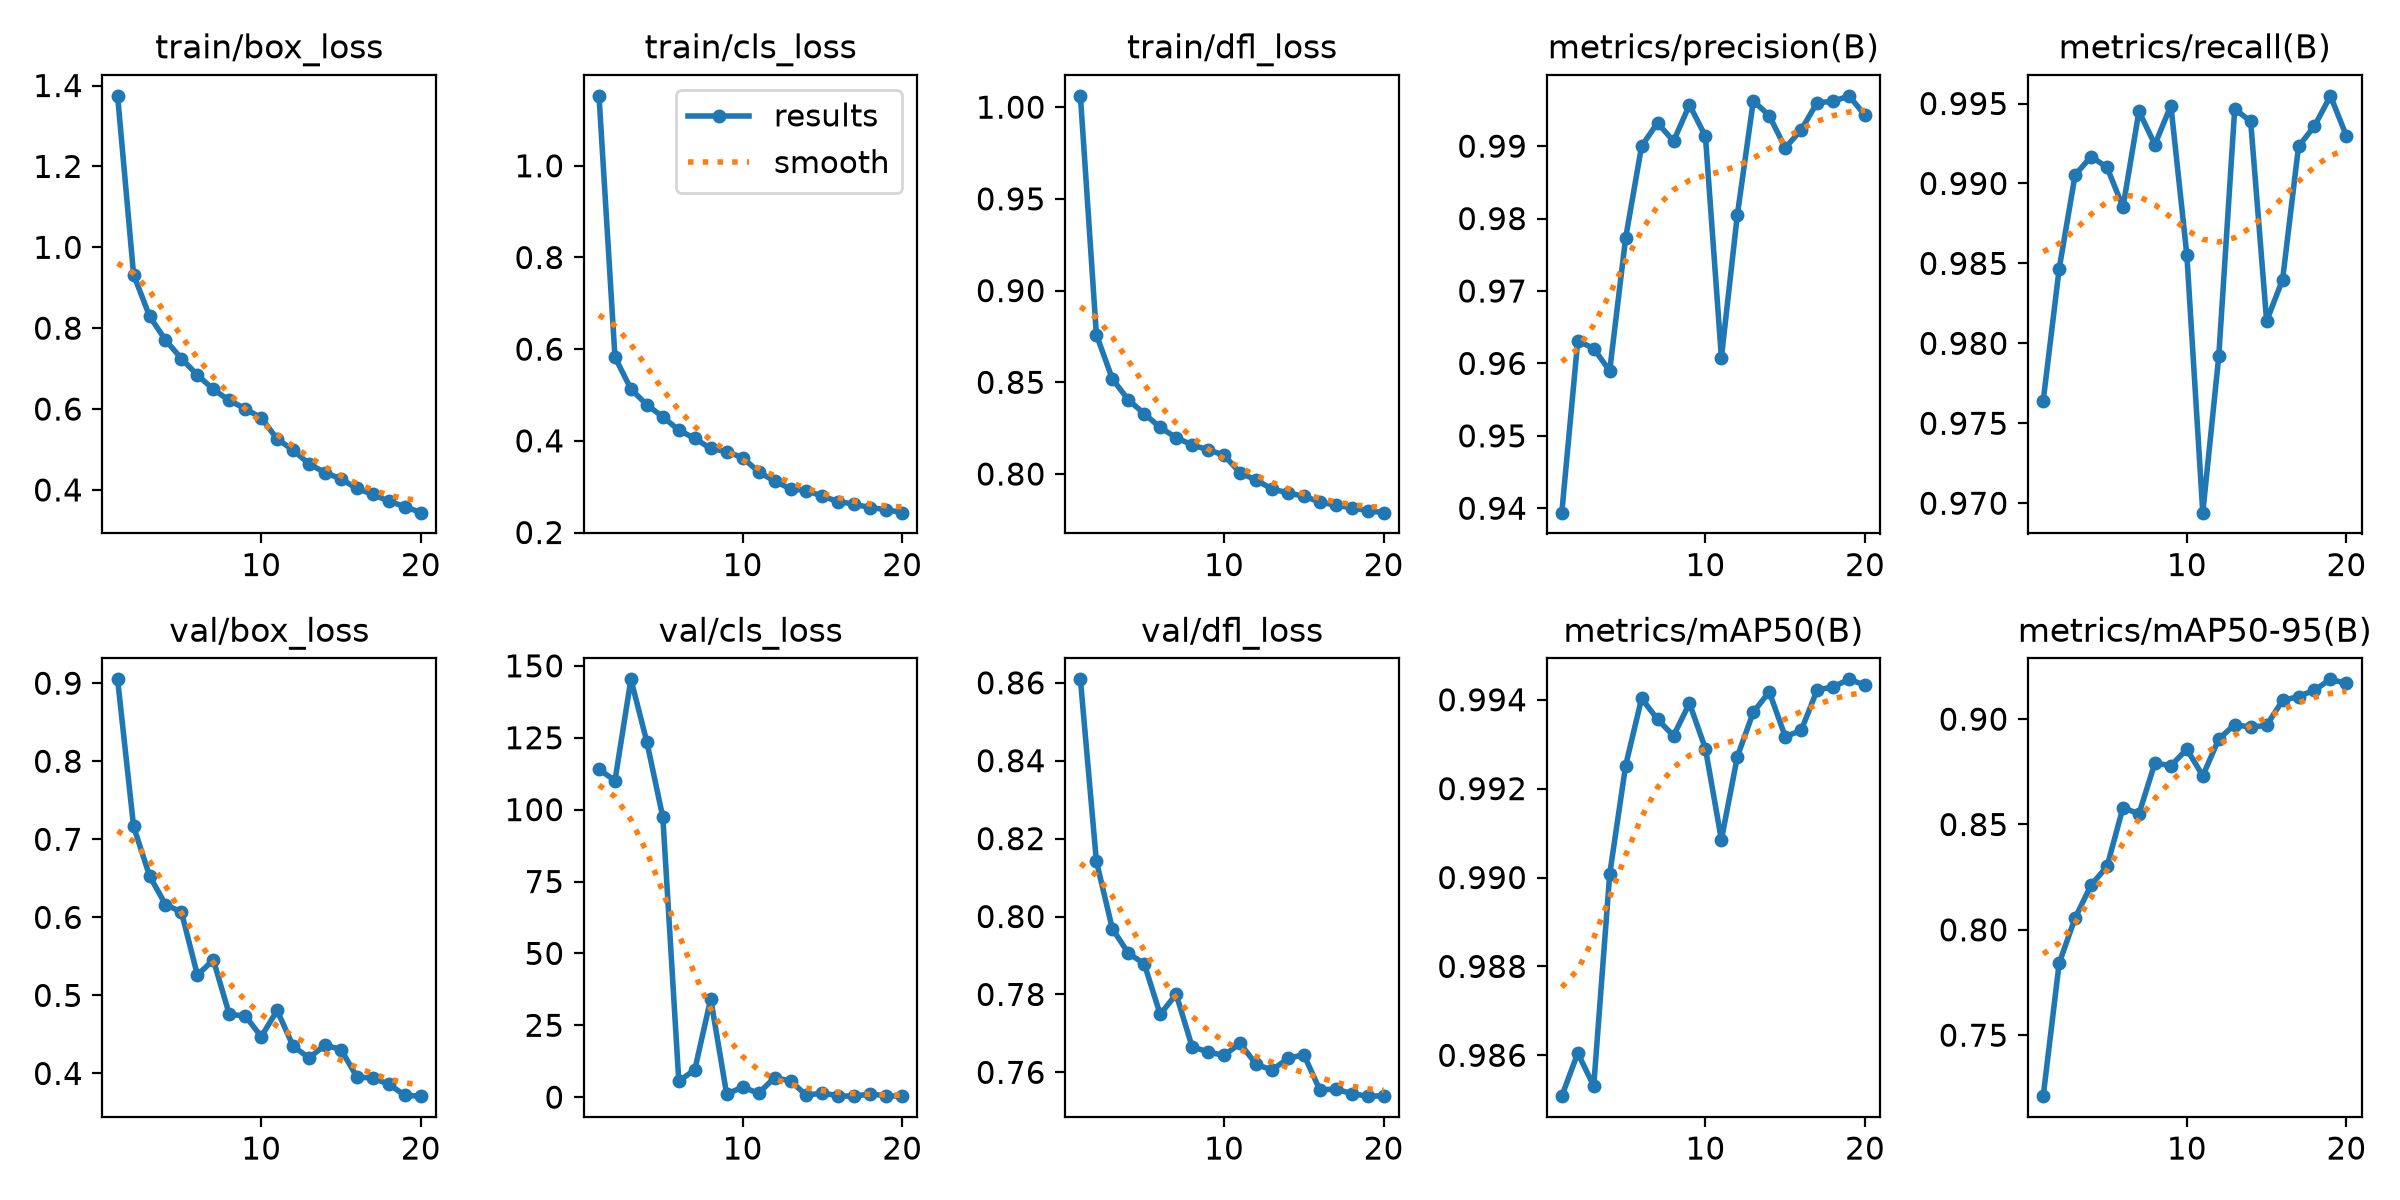
\includegraphics[width=0.92\textwidth]{yolo11n_results.png}
\caption{Entrenamiento de YOLO11n. La validación se satura cerca de 0,99 de mAP50; el test de otros días queda en 0,914.}
\label{fig:curva}
\end{figure*}

La matriz de la Fig.~\ref{fig:matriz} es la de validación que guarda el entrenamiento, no la del test. En ese conjunto el modelo casi no cambia una clase por la otra: la columna de plazas libres cae entera en libre, y la de ocupadas cae 0,99 en ocupada y 0,01 en libre. La columna de fondo, detecciones sin plaza anotada, se reparte 0,67 en libre y 0,33 en ocupada. El fallo no es confundir un auto con un lugar vacío. Es proponer una plaza donde el anotador no puso ninguna. En una cámara fija eso se puede cortar con una máscara de las plazas del predio. Este prototipo no la usa: redescubre la geometría en cada frame.

\begin{figure}[t]
\centering
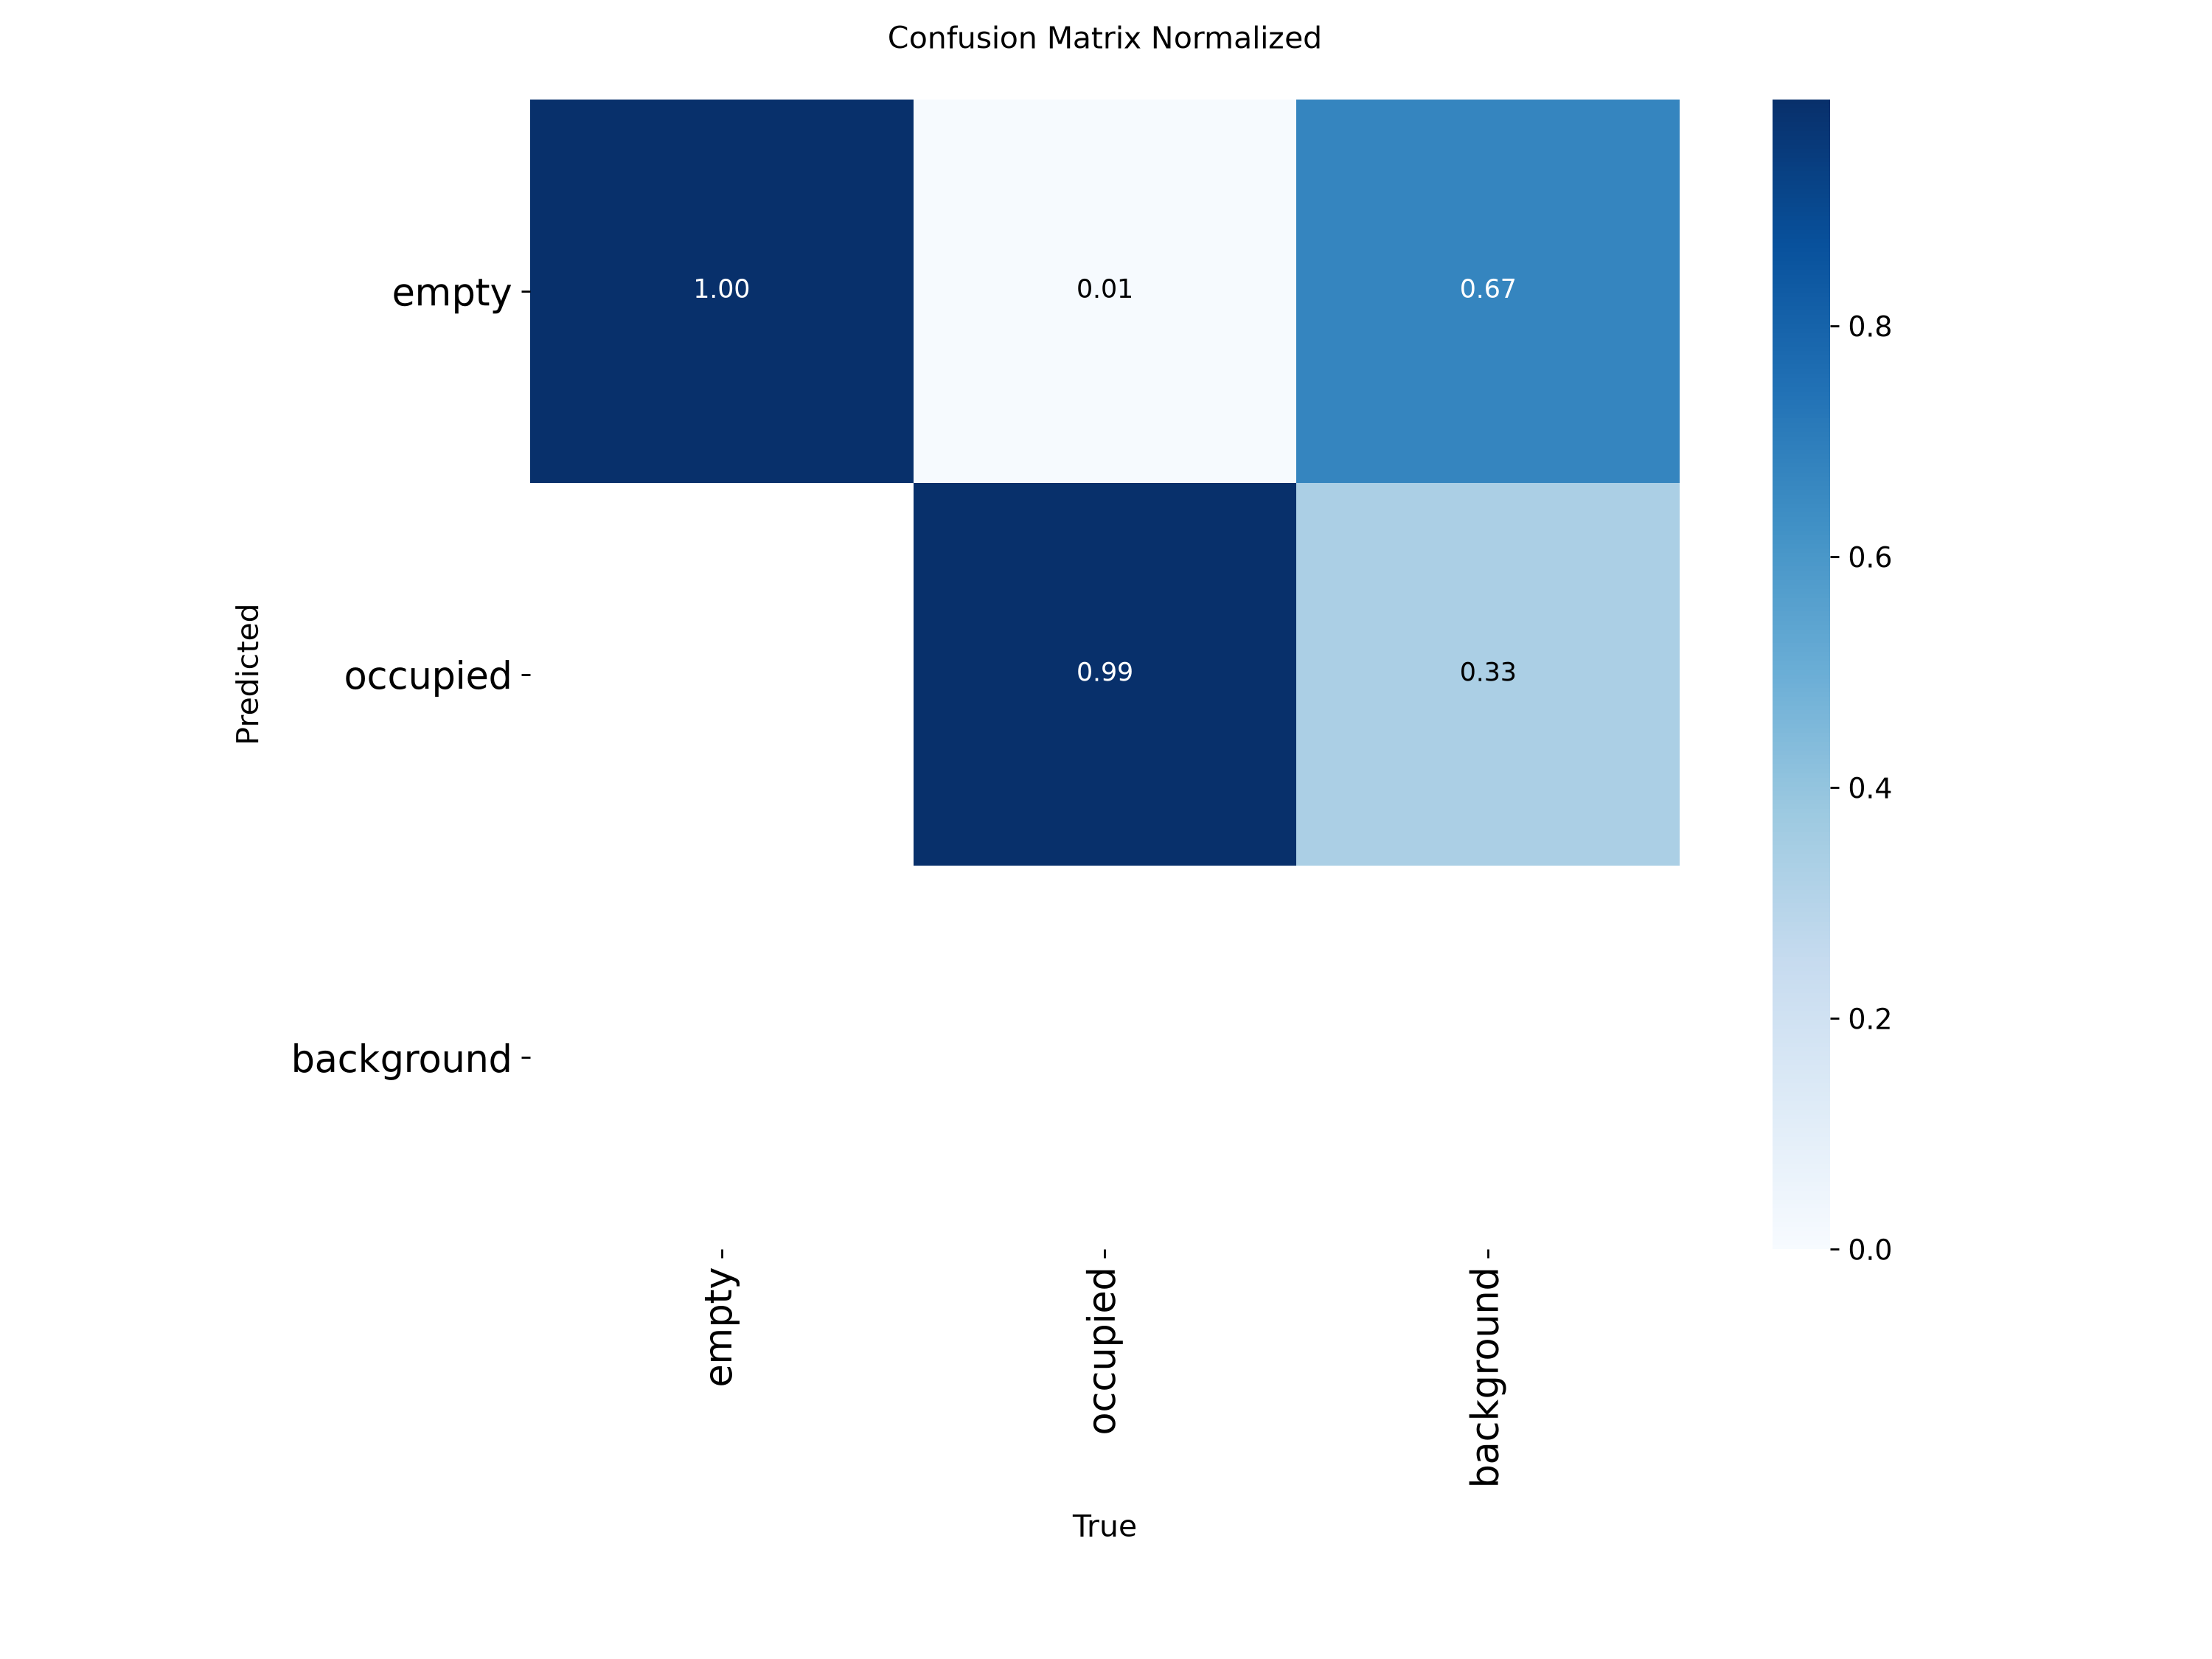
\includegraphics[width=\columnwidth]{yolo11n_confusion.png}
\caption{Matriz normalizada de YOLO11n en validación. Casi no hay intercambio entre libre y ocupada. El fondo concentra las detecciones sin anotación.}
\label{fig:matriz}
\end{figure}

La Fig.~\ref{fig:plazas} es un frame del test. El recuadro de ese frame dice 80 plazas libres y 21 ocupadas. Verde es libre y rojo es ocupada. En la muestra usada para el video, el último frame marcó 25 libres y 15 ocupadas: el número depende de qué porción del predio mire la cámara, no de un total del dataset. El tiempo de esa pasada, con dibujo incluido, fue 24,29\,ms por frame. La latencia de la Tabla~\ref{tab:test} no dibuja.

\begin{figure}[t]
\centering
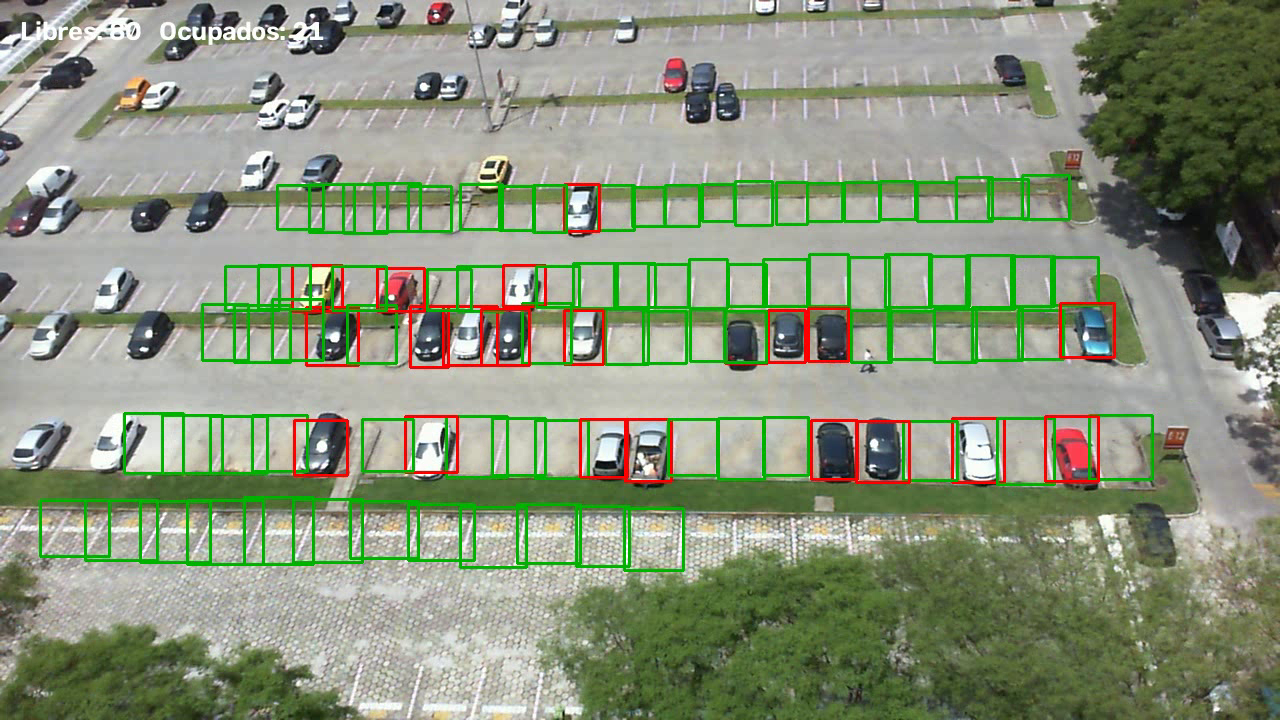
\includegraphics[width=\columnwidth]{plazas.png}
\caption{Frame de test. El detector separa plazas libres (verde) y ocupadas (rojo).}
\label{fig:plazas}
\end{figure}

En el acceso se usó el video de la clase de seguimiento, de 453 frames a 1920$\times$1080. No es la puerta de un estacionamiento: es un cruce urbano, y sirve para probar detección, seguimiento y línea, no para afirmar un conteo de un predio real. El clip termina con 3 ingresos y 1 egreso, o sea un delta de cupo de $-2$. La Fig.~\ref{fig:acceso} es un frame temprano, cuando el contador todavía está en cero, y muestra los identificadores y la trayectoria. La pasada completa, seguimiento incluido, tomó 19,17\,ms por frame.

\begin{figure}[t]
\centering
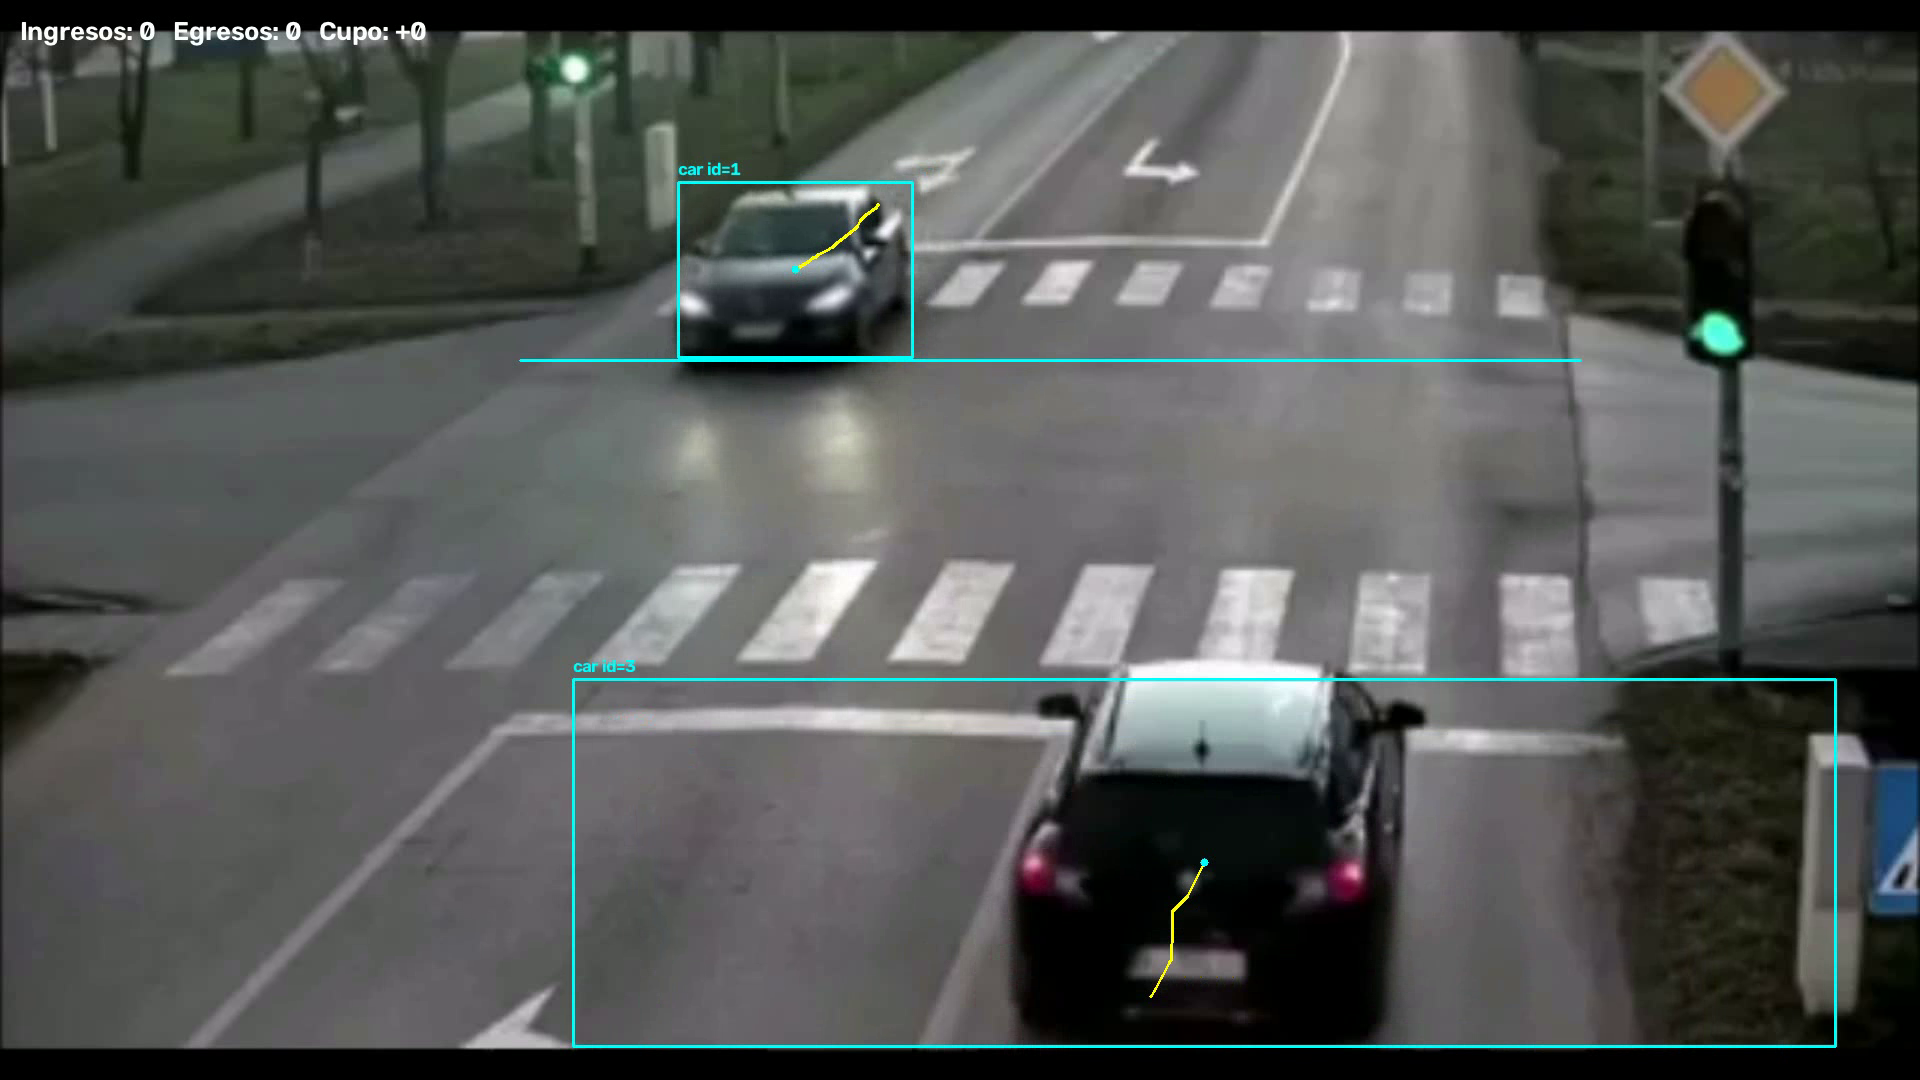
\includegraphics[width=\columnwidth]{acceso.png}
\caption{Acceso con YOLO11s de COCO y ByteTrack. El total del clip es 3 ingresos y 1 egreso.}
\label{fig:acceso}
\end{figure}

\section{Discusión}
Pokhrel y Dao mueven el backbone dentro de YOLOv8 y miden ocupación sobre PKLot \cite{pokhrel2025yolov8pklot}. Acá el cambio de arquitectura es de escala, nano contra small, dentro de YOLO11, y se agrega el flujo de la entrada. No se comparan los mAP con los de ese trabajo: el corte, la caja y la red no son los mismos. Lo que sí se puede afirmar es que, en este corte por día, subir de nano a small no mejora el mAP50 de test.

La validación premia a YOLO11s en mAP50-95 (0,937 contra 0,917) y el test lo castiga. Una lectura posible es que el small ajusta mejor los días que ya vio y generaliza peor a otro día. Veinte épocas pueden no alcanzar para que el small termine de acomodarse, y la paciencia de 5 no cortó la corrida, así que no hubo una meseta temprana que el script haya tomado por convergencia. La regla, igual, mira el test. Con esa regla el nano es el modelo del prototipo.

El desbalance también importa para leer el 0,914. Hay más del triple de plazas libres que ocupadas. Un mAP global alto puede convivir con una clase ocupada en 0,870. Si el producto tiene que decir ``hay lugar'', la precisión de ocupada (0,780) es el número que duele: cada falso ocupado es un lugar que el sistema no ofrece. Un mapa fijo de plazas, multiplicado frame a frame por estas detecciones, atacaría la columna de fondo de la Fig.~\ref{fig:matriz} sin volver a entrenar.

En el acceso, ByteTrack evita el doble conteo solo mientras el identificador sobrevive al cruce. Si el detector pierde el auto justo sobre la línea y el seguidor abre otro id, el mismo vehículo suma dos veces. El video usado no es una barrera: es un cruce de la clase de seguimiento, con la línea calibrada para ese encuadre. Sirve para medir que la cadena detecta, sigue y cambia de semiplano. No sirve para publicar un balance de un estacionamiento real. Los 19,17\,ms por frame incluyen el seguimiento; los 9,83\,ms de la Tabla~\ref{tab:test} son solo la red de plazas.

Juntar las dos ramas en un solo cupo, sin que las cámaras vean el mismo predio y el mismo reloj, mezclaría un inventario con un caudal. Por eso la demo los deja separados: plazas libres y ocupadas por un lado, ingresos y egresos por el otro, y el delta del acceso como lectura aparte.

\section{Conclusiones}
\begin{enumerate}
\item Hace falta detectar cada plaza. Clasificar la imagen entera no dice cuántos lugares libres hay cuando el frame contiene decenas.
\item YOLO11n es el modelo a desplegar en este split: mAP50 de test 0,914 contra 0,891 de YOLO11s, con la misma latencia de unos 10\,ms. Agrandar la red no compró precisión en días no vistos.
\item La validación cerca de 0,99 de mAP50 no es el número del sistema. El corte por día baja el mAP50 a 0,91. Un corte aleatorio habría ocultado ese salto.
\item En validación YOLO11s sí mejora el mAP50-95 (0,937 contra 0,917). La métrica de selección tiene que ser la del test, no la del lazo de entrenamiento.
\item El acceso no necesita un dataset propio. COCO más ByteTrack alcanza para no contar dos veces el mismo vehículo, siempre que el identificador no se rompa al cruzar la línea.
\item Las dos cámaras responden preguntas distintas. El delta de ingresos y egresos no sustituye el conteo de plazas, y en la demo ni siquiera provienen del mismo predio.
\item A 19--24\,ms por frame de punta a punta, en esta GPU, las dos ramas entran en tiempo real. La línea de conteo hay que calibrarla en la cámara verdadera: la de este video está puesta para un cruce de la clase.
\end{enumerate}

El límite principal es de datos de acceso. Falta un video de una barrera real, con la línea medida sobre ese encuadre, para saber si el sentido configurado coincide con la entrada del predio.

\bibliographystyle{IEEEtran}
\bibliography{references}

\end{document}
